In this experiment the hierarchical clustering is used because of its characteristic in estimation of the number of clusters, as described in section \ref{sec:hierarchical_cluster_estim}.
In order to simulate or import real-world sensor, source and volume conduction head model required to generate the real lead-field we used an open source software package MATLAB-based toolbox named FieldTrip \cite{Oostenveld2011}.

EEG lead-field is obtained using 32 standard electrodes and utilising three different volume conduction head models of three-layer concentric spheres, realistic three-layer with inflated cortical sheet obtained by boundary element
methods and realistic three-layer with highly-folded cortical sheet obtained by SPM8 software \cite{SPM}.
Realistic head models are obtained by imposing anatomical constraint, which is provided by MRI\footnote{\emph{Magnetic Resonance Imaging}}.

Similarly, for MEG lead-field generating, 32 standard sensors closest to the previously selected 32 EEG standard electrodes are selected and single sphere, realistic single layer with inflated and highly-folded cortical sheets are used as volume conduction head models.
The sensor model, three-compartment (brain, skull, and scalp) volume conduction head model (analytical and realistic), and source model (spherical and realistic) are shown in figure \ref{fig:Sensor_vol_Source}. 
\begin{figure}[!b]
\centering
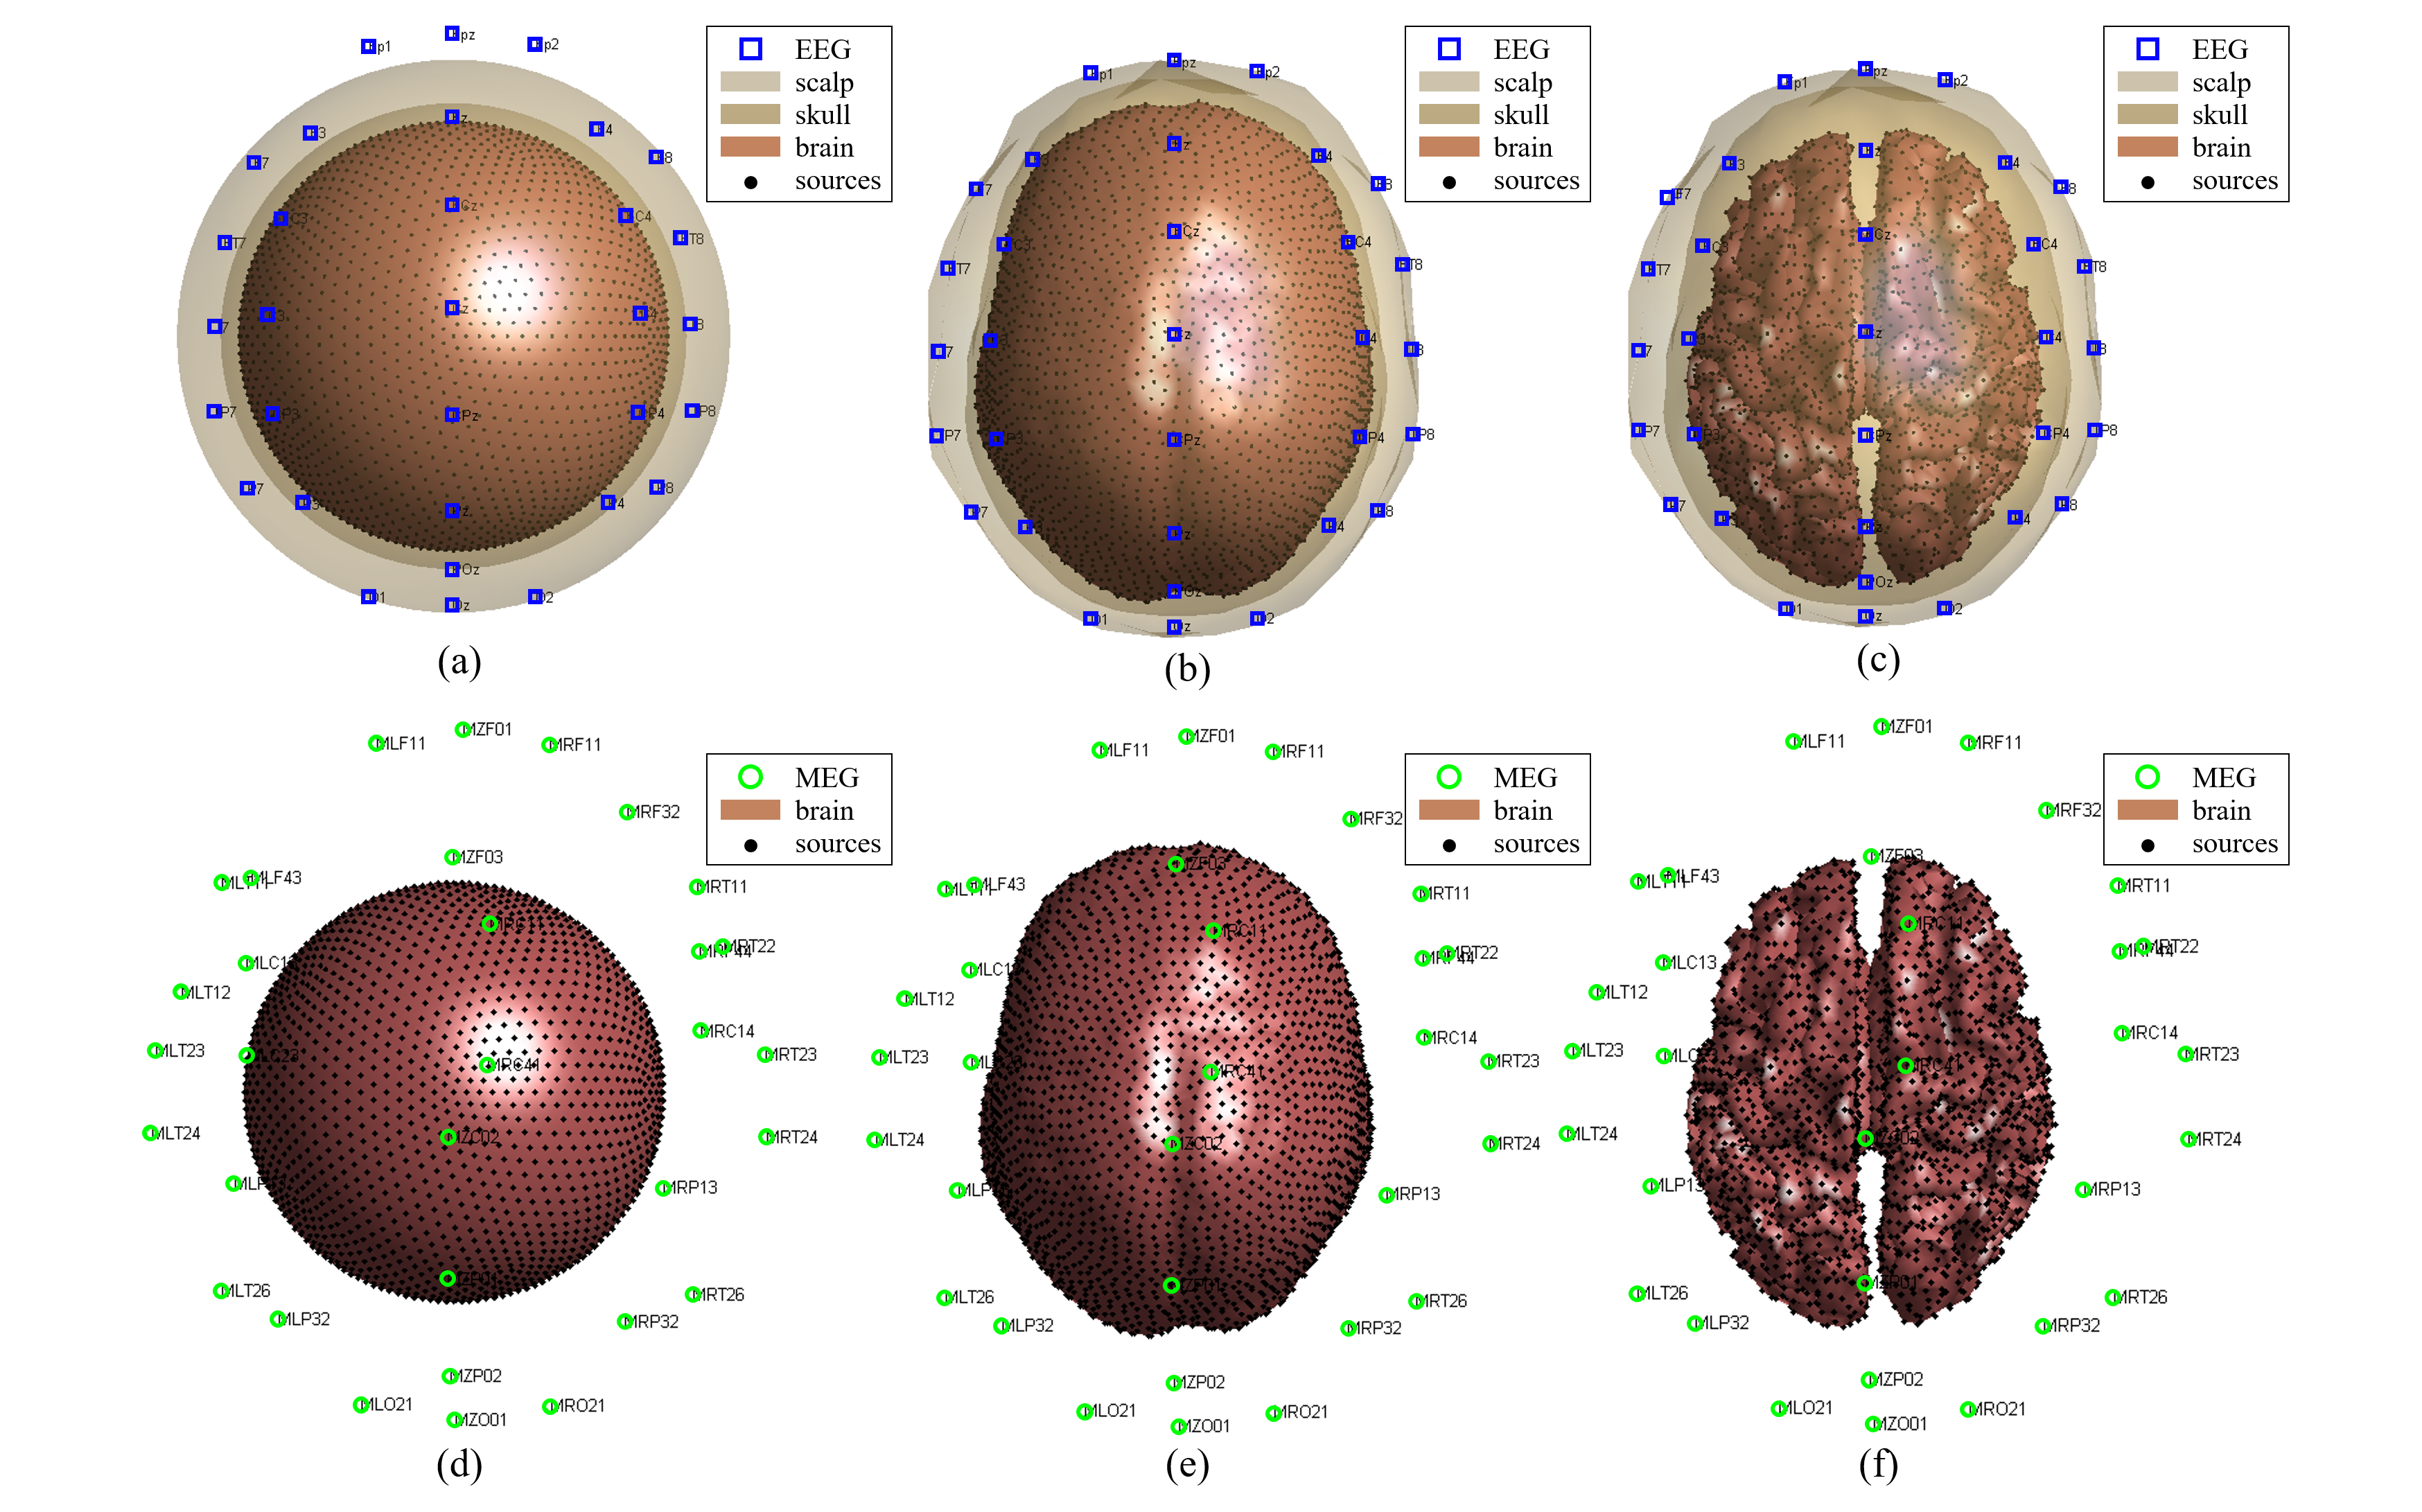
\includegraphics[width=1\textwidth,keepaspectratio]{images/Sensor_vol_Source.png} % width=0.5\textwidth  scale=0.49
\centering
\caption{Different geometrical models of the EEG/MEG experiment: 1- Spherical (a,d), realistic inflated (b,e), and realistic highly-folded (c,f) source models; 2- EEG (a,b,c), and MEG (d,e,f) sensor models; 3- Three-layer concentric spheres (a), realistic three-layer (b,c), single sphere (d), and realistic single layer (e,f) volume conduction head models.}
\label{fig:Sensor_vol_Source}
\end{figure}
\FloatBarrier
%------------------------------------------------------
%\subsubsection{Sparsity level in a clustered blocks compared to the initial unclustered blocks}
\paragraph{Block-ERC in clustered representation}
As explained in Section \ref{sec:Sparsity level for clustered blocks of a dictionary}, generally, in transforming the $\myBSLqpTxt$, which is determined by Block-ERC, into the conventional sparsity level, different types of sparsity levels can be appeared, e.g., minimum sparsity level 
%in the most pessimistic case 
$\mySLTxt_{min}$, and maximum sparsity level 
%in the most pessimistic case 
$\mySLTxt_{max}$.
%, minimum sparsity level in the most optimistic case $\mySLTxt^{opt}_{min}$, and maximum sparsity level in the most optimistic case $\mySLTxt^{opt}_{max}$.
On the other hand, as described earlier in the Section \ref{sec:hierarchical_cluster_estim}, number of branches in a clustering level with maximum inter-node distance in a clustering tree resulted from a hierarchical clustering algorithm can be used as an estimation of the number of clusters of a dictionary.

Assume the sparsity level computed in the clustering level corresponding to the maximum inter-node distance in the clustering tree is shown by $\mySLTxt_2$, whereas the sparsity level computed for the lead-field without clustering is called $\mySLTxt_1$.
In order to investigate the effect of clustering the coherent blocks of the lead-field on sparsity levels, we compute the relative change quantity, i.e., $(\mySL_2(\myPhi) \sm \mySL_1(\myPhi)) {/} \mySL_1(\myPhi)$.

In figure \ref{fig:EMEG-LF-clustering-SL}, the relative change of sparsity levels $\mySLTxt_{min}$, and $\mySLTxt_{max}$ is shown.
%, $\mySLTxt^{opt}_{min}$, and $\mySLTxt^{opt}_{max}$ is shown.
In addition, the experiment is repeated for two modalities of EEG and MEG, and three head models with spherical, realistic inflated and realistic highly-folded cortical sheets.

As it can be seen in figure \ref{fig:EMEG-LF-clustering-SL}, by clustering coherent blocks of the lead-field (whether EEG/MEG or spherical/realistic cortical sheet) using the proposed Block-MCC$_{2,2}$, all sparsity levels significantly increase, especially $\mySLTxt_{max}$.
% and $\mySLTxt^{opt}_{max}$.
Hence, clustering coherent blocks of lead-field using the proposed Block-MCC$_{q,p}$ coherence measure leads to improved Block-ERC.

%In addition to the segmentation effect mentioned in previous part, the relative improvement of $\mySLTxt^{pes}_{min}$, $\mySLTxt^{pes}_{max}$, $\mySLTxt^{opt}_{min}$, and $\mySLTxt^{opt}_{max}$ in the estimated clustering level in comparison to the last level of clustering where the number of clusters is equal to the number of blocks, is shown in figure \ref{fig:EMEG-LF-clustering-SL} as bar charts, which indicates a significant increase on values, i.e., clustering coherent blocks of leadfield results in weakened recovery conditions.
\begin{figure}[!b]
\centering
\includegraphics[width=0.9\textwidth,keepaspectratio]{images/EMEG-LF-clustering-SL.png} % width=0.5\textwidth  scale=0.49
\centering
\caption{Relative increase of sparsity levels $\mySLTxt_{min}$, $\mySLTxt_{max}$, 
%$\mySLTxt^{opt}_{min}$, and $\mySLTxt^{opt}_{max}$, 
when clustering the coherent blocks of lead-field, repeated for two modalities of EEG and MEG, and three head models with spherical, realistic inflated and realistic highly-folded cortical sheets.}
\label{fig:EMEG-LF-clustering-SL}
\end{figure}
\FloatBarrier
%------------------------------------------------------
\paragraph{EEG/MEG source space segmentation}
As described in Section \ref{sec:EMEG segmentation}, clustering the coherent blocks of the lead-field matrix results in some brain regions, because each block of the lead-field correspond to \myhl{a single source position in the source space.}
Then, coherent source positions form brain regions, where, coherency is defined by the Block-MCC$_{q,p}$ coherence measure applied on the bocks of the lead-field.

The results of clustering coherent source positions using EEG and MEG lead-field, and for three head models with spherical, realistic inflated and realistic highly-folded cortical sheets are shown in figure \ref{fig:EMEG-LF-clustering-regions}. 
Although, in this experiment the number of clusters or brain regions is estimated from the clustering tree, but since there is a series of clustering structures in the hierarchical clustering analysis, by introducing extra information to the problem about the number of brain regions, there would be the possibility of having different brain regions.
In other words, the resulted brain regions in figure \ref{fig:EMEG-LF-clustering-regions} are not fixed and can be adapted based on the number of regions.
In addition, the resulted brain regions are a function of Block-MCC$_{q,p}$ and inter-cluster distance method.


%By clustering the blocks of the leadfield matrix, coherent sources form clusters, hence brain regions appear as described in Section \ref{sec:EMEG segmentation} and the number of clusters can be estimated by counting the number of intersections of a horizontal line with the dendrogram in an area where there is the maximum distance between adjacent nodes.

%Using Block-MCC$_{1,\infty}$ as the similarity measure and the complete method as the algorithm for computing the distance between clusters, the brain source space segmentation resulted from EEG leadfield clustering in three cases of one spherical and two realistic volume conduction head models can be seen in figure \ref{fig:EMEG-LF-clustering_regions}(a), (b), and (c), respectively.
%As it can be seen in figure \ref{EMEG-LF-clustering-regions}(a), with the help of dendrogram it is possible to estimate the number of clusters and the clustering structure.
%Similar results are obtained from MEG leadfield, which are shown in figure \ref{EMEG-LF-clustering-regions}(d), (e) and (f).
\begin{figure}[!b]
\centering
\includegraphics[width=1\textwidth,keepaspectratio]{images/EMEG-LF-clustering-regions.png} % width=0.5\textwidth  scale=0.49
\centering
\caption{Brain source space segmentation, when clustering the coherent blocks of lead-field, repeated for two modalities of EEG and MEG, and three head models with spherical, realistic inflated and realistic highly-folded cortical sheets.}
\label{fig:EMEG-LF-clustering-regions}
\end{figure}
\FloatBarrier
%------------------------------------------------------
\paragraph{Comparison to the conventional lobes of the brain}
In order to compare the resulted brain source space segmentation in a specific clustering level to the conventional lobes of the brain, the closest boundaries to the conventional boundaries are shown in figure \ref{fig:Atlas}(a) and (b).

The brain segmentation and boundaries resulted from EEG, and MEG lead-fields are shown in figure \ref{fig:Atlas}(a), and (b), respectively.
The anatomical lobes and the functional areas of the brain are shown in figure \ref{fig:Atlas}(c).

Therefore, using the proposed framework, i.e., clustering coherent blocks of the lead-field with the help of the proposed Block-MCC$_{q,p}$ coherence measure, the conventional structural and functional brain lobes can be divided into subject-specific refined regions.
\begin{figure}[!b]
\centering
\includegraphics[width=1\textwidth,keepaspectratio]{images/Atlas.png} % width=0.5\textwidth  scale=0.49
\centering
\caption{The proposed subject-specific brain source space segmentation, using (a) EEG, and (b) MEG lead-fields, compared to (c) the conventional anatomical and functional brain lobes.}
\label{fig:Atlas}
\end{figure}
\FloatBarrier